\documentclass[a4paper]{article}

\setlength{\oddsidemargin}{-1in}
\addtolength{\oddsidemargin}{0.05 \paperwidth}
\setlength{\evensidemargin}{-1in}
\addtolength{\evensidemargin}{0.05 \paperwidth}
\setlength{\textwidth}{0.9 \paperwidth}

\setlength{\topmargin}{-0.75in}
\addtolength{\topmargin}{0.05 \paperheight}
\setlength{\textheight}{\paperheight}
\setlength{\headheight}{0in}
\setlength{\headsep}{0in}
\setlength{\footskip}{0in}

\usepackage[T1]{fontenc}
\usepackage[utf8]{inputenc}
\usepackage[german]{babel}

\usepackage[default,scale=1.7]{opensans}
\usepackage[scaled=2.6]{beramono}
\linespread{1.9}

\usepackage{url}
\usepackage{graphicx}

\usepackage{grid-system}

\usepackage{color}
\definecolor{freifunkpink}{RGB}{215,0,73}
\definecolor{freifunkyellow}{RGB}{255,191,0}
\definecolor{lightgrey}{RGB}{220,220,220}

\usepackage{enumitem}
\setlist[itemize]{leftmargin=*}

\begin{document}
\thispagestyle{empty}

\begin{center}
  \Huge \textit{\textbf{\textcolor{freifunkpink}{Freies WLAN für Ihre Gäste}}} \\
  \vspace{0.6cm}
  \large Wollen Sie ihren Kunden kostenloses Internet ermöglichen - ohne großen Aufwand und Kosten?\\
  Willkommen beim gemeinnützigen Freifunk-Projekt!\\
  \normalsize

  \vspace{1.25cm}
  \hspace*{-0.05 \paperwidth}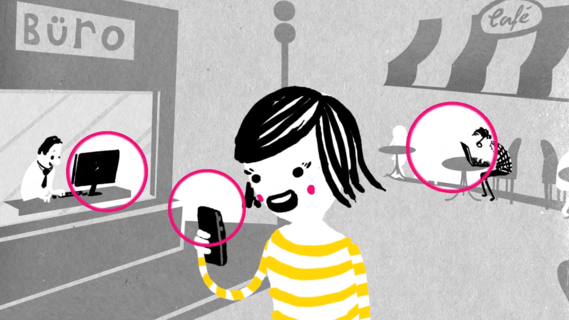
\includegraphics[width=\paperwidth]{../images/city_center}
\end{center}

\vspace{0.6cm}

\begin{Row}
  \begin{Cell}{1}
    \textbf{Was ist Freifunk?}\\
    Das spendenfinanzierte, gemeinnützige Freifunk-Netz ist unbeschränkt nutzbar, unzensiert und für Betreiber und Nutzer kostenlos. Mit wenigen Euro Einmalkosten für Router und Kabel sind Sie dabei. Danach ist Schluss mit dem Herausgeben ihres WLAN-Passwortes.
  \end{Cell}
  \begin{Cell}{1}
    \textbf{Ihre Vorteile} \vspace*{-0.18cm}
    \begin{itemize}
      \item[\textcolor{freifunkpink}{\Large$\bullet$}] höhere Attraktivität ihrer Geschäftsräume für Kunden
      \vspace*{-0.3cm}
      \item[\textcolor{freifunkpink}{\Large$\bullet$}] keine laufenden Kosten für Betreiber und Nutzer\vspace*{-0.3cm}
      \item[\textcolor{freifunkpink}{\Large$\bullet$}] keine Nutzerregistrierung
      \vspace*{-0.3cm}
      \item[\textcolor{freifunkpink}{\Large$\bullet$}] unsere Community aus freiwilligen Helfern unterstützt Sie gerne bei technischen Fragen und beim Aufbau
    \end{itemize}
  \end{Cell}
\end{Row}

\newpage

\thispagestyle{empty}

\begin{center}
  \Huge \textit{\textbf{\textcolor{freifunkpink}{Freifunk für alle}}} \\
  \vspace{0.6cm}
\end{center}

\begin{Row}[cellsep=0.75cm]
  \begin{Cell}{1}
      Durch das Anbieten eines Internetzugangs über das Freifunk-Netz können Rechtsverstöße der Benutzer nicht auf Sie zurückverfolgt werden, da das Freifunk-Netz von ihrem Internetanschluss technisch getrennt ist.
      Bei der unkomplizierten Installation unterstützen wir Sie gerne ehrenamtlich. Zusätzlich können Sie durch weitere Router auch bisher internetfreie Bereiche ihres Anwesens (z.B. der Außenbereich eines Cafés) mit WLAN versorgen und sich mit anderen Freifunk-Routern in Ihrer Nähe verbinden, wodurch eine unabhängige Netzwerkinfrastruktur entsteht. Dadurch unterstützen Sie den Grundgedanken von Freifunk: ein flächendeckendes, dezentrales und freies WLAN-Netz, das es Menschen an möglichst vielen Orten ermöglicht, untereinander zu kommunizieren und einen unkomplizierten Zugang zum Internet zu erhalten. Über 300 Firmen und Privatleute, sowie Flüchtlingsunterkünfte sind schon dabei.
      Wollen Sie auch ein Punkt auf unserer Karte sein? https://darmstadt.freifunk.net/karte/

      \vspace{1cm}


      \begin{center}
        Bei weiteren Fragen erreichen Sie uns per E-Mail unter:\\
        info@darmstadt.freifunk.net

        \vspace{1cm}
        Mehr über Ihre lokale Freifunk-Initiative erfahren sie unter:\\
        \vspace{0.5cm}
        \large https://darmstadt.freifunk.net/
      \end{center}
      \vspace{2cm}


  \end{Cell}
\end{Row}

\vspace{0.8cm}
\begin{center}
  \hspace*{-0.05 \paperwidth}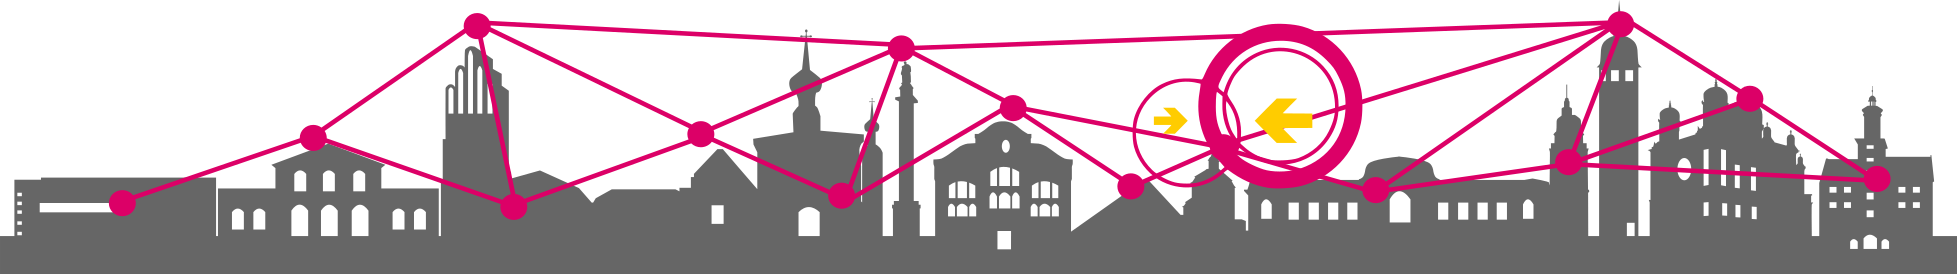
\includegraphics[width=\paperwidth]{../images/footer_skyline_notext.png}
\end{center}


\end{document}
